% Copyright (c) 2026 CorrectBrain
% SPDX-License-Identifier: MIT

\PassOptionsToPackage{dvipsnames,svgnames,x11names}{xcolor}
\documentclass[tikz,border=8pt]{standalone}
\usetikzlibrary{arrows.meta,positioning,calc,shapes,shadows,decorations.pathmorphing,shapes.geometric,backgrounds,decorations.markings,decorations.pathreplacing,decorations.text,fit,shapes.misc,shapes.arrows,matrix,bending,3d,chains,intersections,shapes.symbols,svg.path,shapes.multipart,snakes,shapes.callouts,angles,quotes}
\providecolor{gold}{RGB}{212,175,55}
\providecolor{silver}{RGB}{192,192,192}
\providecolor{bronze}{RGB}{205,127,50}
\providecolor{darkblue}{RGB}{0,0,139}
\providecolor{lightblue}{RGB}{173,216,230}
\providecolor{darkgreen}{RGB}{0,100,0}
\providecolor{lightgreen}{RGB}{144,238,144}
\providecolor{darkred}{RGB}{139,0,0}
\providecolor{navy}{RGB}{0,0,128}
\providecolor{skyblue}{RGB}{135,206,235}
\providecolor{beige}{RGB}{245,245,220}
\providecolor{cream}{RGB}{255,253,208}
\usepackage{amsmath}
\usepackage{amssymb}
\usepackage{fontawesome5}
\usetikzlibrary{fadings,shadows.blur,patterns,patterns.meta}

\usepackage{amsmath}
\usepackage{amssymb}
\usepackage{fontawesome5}

\providecolor{gold}{RGB}{212,175,55}
\providecolor{silver}{RGB}{192,192,192}
\providecolor{bronze}{RGB}{205,127,50}
\providecolor{darkblue}{RGB}{0,0,139}
\providecolor{lightblue}{RGB}{173,216,230}
\providecolor{darkgreen}{RGB}{0,100,0}
\providecolor{lightgreen}{RGB}{144,238,144}
\providecolor{darkred}{RGB}{139,0,0}
\providecolor{navy}{RGB}{0,0,128}
\providecolor{skyblue}{RGB}{135,206,235}
\providecolor{beige}{RGB}{245,245,220}
\providecolor{cream}{RGB}{255,253,208}

\definecolor{cssblue}{RGB}{20, 100, 180}
\definecolor{nativeteal}{RGB}{0, 150, 136}
\definecolor{containergray}{RGB}{240, 240, 245}
\definecolor{warnred}{RGB}{211, 47, 47}
\definecolor{mathpurple}{RGB}{123, 31, 162}

\begin{document}
\begin{tikzpicture}[
    font=\sffamily,
    bubble/.style={draw=black!30, fill=white, rounded corners=8pt, blur shadow={shadow opacity=15}, inner sep=10pt},
    pixel/.style={draw=white, line width=0.5pt}
]

% =========================================================================
% Top Section: Titles (Absolute Layout)
% =========================================================================
\node[font=\Huge\bfseries, color=black!80] at (0, 18) {The Mathematics of \texttt{width: 100\%}};
\node[font=\Large, color=black!60] at (0, 17) {Why scaling low-resolution images forces extreme pixelation};

% =========================================================================
% Section 1: The Native Image Group (Left, centered at X = -6)
% =========================================================================
\node[font=\Large\bfseries, nativeteal, anchor=south] at (-6.1155,13.3066) {\faImage\ Native Image File};
\node[font=\small, text width=5cm, align=center, black!70, anchor=south] at (-6.077,11.6136) {Low resolution (e.g., $100 \times 100$ px)\\Contains exactly $10,000$ unique pixels of data.};

% Native Image Box: mathematically 2x2 units [(-7,7) to (-5,9)]
\fill[nativeteal!15, rounded corners=2pt, blur shadow] (-7, 7) rectangle (-5, 9);
\draw[step=0.25, nativeteal!40, line width=0.3pt] (-7, 7) grid (-5, 9);
\draw[thick, nativeteal, rounded corners=2pt] (-7, 7) rectangle (-5, 9);

% Dimension line & label
\draw[<->, nativeteal, thick] (-7, 6.6) -- (-5, 6.6);
\node[nativeteal, font=\small, anchor=north] at (-6, 6.2) {$W_{native} = 100px$};

% =========================================================================
% Section 2: The Web Container Group (Right, centered at X = 6)
% =========================================================================
\node[font=\Large\bfseries, cssblue, anchor=south] at (6, 14.5) {\faIcon{mobile-alt}\ Web Container};
\node[font=\small, text width=6.5cm, align=center, black!70, anchor=south] at (6, 13.5) {High-density Display (e.g., $400 \times 400$ px)\\Requires $160,000$ pixels to fill the space.};

% Outer Device Bezel: [(1.5, 3.5) to (10.5, 12.5)]
\fill[fill=gray!15, rounded corners=8pt, drop shadow] (1.5, 3.5) rectangle (10.5, 12.5);
\draw[gray!40, line width=0.8pt, rounded corners=8pt] (1.5, 3.5) rectangle (10.5, 12.5);

% Inner Screen: mathematically 8x8 units [(2, 4) to (10, 12)]
\fill[white] (2, 4) rectangle (10, 12);
\draw[step=0.25, cssblue!15, line width=0.1pt] (2, 4) grid (10, 12);
\draw[thick, cssblue, dashed] (2, 4) rectangle (10, 12);

% Dimension line & label
\draw[<->, cssblue, thick] (2, 3.1) -- (10, 3.1);
\node[cssblue, font=\small, anchor=north] at (6, 2.7) {$W_{container} = 400px$};

% =========================================================================
% Connection & Action (Center X = 0, Center Y = 8)
% =========================================================================
\draw[-Stealth=3mm, line width=3pt, cssblue] (-4.5, 8) -- (1.2, 8);
\node[font=\ttfamily\Large\bfseries, cssblue, anchor=south] at (-1.5, 8.5) {\texttt{width: 100\%;}};
\node[bubble, text width=4cm, align=center] at (-1.5, 3.5) {\textbf{The Command:}\\ "Stretch my 100px of data to fill this 400px void."};

% =========================================================================
% Section 3: The Mathematical Deficit
% =========================================================================
\node[font=\Huge\bfseries, mathpurple] at (0, 0) {\faCalculator\ The Mathematical Deficit};

\node[bubble, text width=16cm, align=left] at (0, -2.5) {
    \textbf{1. Scale Factor (1D):} $S = \frac{W_{container}}{W_{native}} = \frac{400px}{100px} = 4$\\[3pt]
    \textbf{2. Area Multiplier (2D):} Since images are 2D grids, the total pixel requirement scales quadratically:\\
    $Area = S^2 = 4^2 = \mathbf{16}$\\[3pt]
    \textbf{3. The Gap:} The browser needs $160,000$ pixels, but only has $10,000$ real pixels. It must \textbf{invent 15 fake pixels} for every 1 real pixel.
};

% =========================================================================
% Section 4: Interpolation Algorithms (Scale Factor 4 Mapping)
% =========================================================================
\node[font=\Large\bfseries, warnred] at (0, -6.5) {\faExclamationTriangle\ How Browsers "Invent" Pixels (Interpolation Algorithms)};

% 1. Original Data (Top Center, mathematically 1x1 area)
\node[font=\bfseries, text width=4cm, align=center] at (0, -8) {Original Data\\(1 Pixel)};
\fill[nativeteal!80, rounded corners=1pt, blur shadow] (-0.5, -10) rectangle (0.5, -9);
\draw[very thick, nativeteal, rounded corners=1pt] (-0.5, -10) rectangle (0.5, -9);
\node[font=\small, text width=3cm, align=left, black!70, anchor=west] at (0.6722,-9.4422) {1 real pixel of\\source data.};

% Branch Arrows starting strictly outside the 1x1 pixel box and routing cleanly to algorithm titles
\draw[-Stealth=3mm, line width=1.5pt, gray!70] (0, -10) -- (-5, -12.2);
\draw[-Stealth=3mm, line width=1.5pt, gray!70] (0, -10) -- (5, -12.2);

% 2. Nearest Neighbor Outcome (Bottom Left, 4x4 area = 16 sub-pixels)
\node[font=\bfseries, text width=5.5cm, align=center] at (-5, -13) {Nearest Neighbor\\(CSS: \texttt{image-rendering: pixelated})};
\foreach \x in {-7,-6,-5,-4} {
    \foreach \y in {-18,-17,-16,-15} {
        \fill[nativeteal!80] (\x, \y) rectangle (\x+1, \y+1);
        \draw[white, thick] (\x, \y) rectangle (\x+1, \y+1);
    }
}
\draw[thick, warnred] (-7, -18) rectangle (-3, -14);
\node[font=\small, text width=5cm, align=center, black!70] at (-5.0193,-19.0188) {Duplicates the original pixel color exactly. Causes "blocky" artifacts.};

% 3. Bicubic Outcome (Bottom Right, 4x4 area = smooth gradient blend)
\node[font=\bfseries, text width=4.5cm, align=center] at (5, -13) {Bicubic\\(Default Browser Behavior)};
\shade[inner color=nativeteal!90, outer color=nativeteal!10] (3, -18) rectangle (7, -14);
\draw[thick, warnred] (3, -18) rectangle (7, -14);
\node[font=\small, text width=4.5cm, align=center, black!70] at (4.9807,-19.0188) {Averages surrounding colors. Causes "muddy" or blurry artifacts.};

% =========================================================================
% Background Layer (Solid White Canvas & Mathematically Aligned Zoom Frustum)
% =========================================================================
\begin{pgfonlayer}{background}
    \fill[white] (current bounding box.south west) rectangle (current bounding box.north east);
    % Zoom Frustum: Connects Native Image right corners to Web Container left screen corners
    \fill[gray, opacity=0.1] (-5, 9) -- (2, 12) -- (2, 4) -- (-5, 7) -- cycle;
\end{pgfonlayer}

\end{tikzpicture}
\end{document}
